%%%%%%%%%%%%%%%%%%%%% chapter.tex %%%%%%%%%%%%%%%%%%%%%%%%%%%%%%%%%
%
% sample chapter
%
% Use this file as a template for your own input.
%
%%%%%%%%%%%%%%%%%%%%%%%% Springer-Verlag %%%%%%%%%%%%%%%%%%%%%%%%%%
%\motto{Use the template \emph{chapter.tex} to style the various elements of your chapter content.}

% Chapter Template

\chapter{The Mathematical perspective} % Main chapter title

\label{Chapter3} % Change X to a consecutive number; for referencing this chapter elsewhere, use \ref{ChapterX}


%----------------------------------------------------------------------------------------
%	SECTION 1
%----------------------------------------------------------------------------------------

\section{Introduction}

In this chapter a overall mathematical introduction to the field of computational fluid dynamics is given. There are several
posibilities to classify and structure the wide field of CFD. In most literature this is done by focusing on the physical properties
of the fluid models itself e.g. Date2005 resulting in categories like incompressible or compressible fluid dynamics. Since the focus of this
report is not on the physical description of fluids, we will take a different approach and structure the report by the domain discretizations
schemes itself which result in the later Chapters 3 "Mesh-based Methods" and Chapter 4 "Mesh-free Methods". First of all a
brief destinction is made between mesh-based and mesh-free methods. These destinction is followed through the entire chapter
and will conclude in detailed descriptions of both methods given in Chapter 3 and Chapter 4. Afterwards the governing physical Navier-Stokes
equations of CFD are given and explained in detail.
For further reading please refer to Date2005, Cebeci2005, Toro2009 and for a comprehensive overview of the mathematical notations in CFD please refer to Aris1989.

\section {Numerical simulation proceedings}
Before diving into the physical world of CFD we first take a look at the general approach to solving a physical problem with a numerical simulation. By understanding this process we can lay out the Chapter in a more structured way. Figure \ref{fig:CFDSimProcess} shows this general process for a fluid flow problem and begins with the physical problem in the real world. Before even considering any kind of
computer program or mathematical equation, the physical phenomena that are involved or might appear in the real world have to be understood. Some important examples for this like \emph{turbulent flow} were given in Chapter \ref{Chapter2}. From this point on, one needs to abstract from nature in order to define a computable model. Conscious decisions have to be made whether the apprehended phenomena are relevant enought to
be involved in the mathematical modelling or not. At the beginning of the mathematical modelling process this Chapter will describe in Section \ref{sec:mathperspective} two major and different \textbf{perspectives} in how a observer can perceive a fluid flow. This \textbf{Eulerian} or \textbf{Lagrangian} perspective leads to different mathematical equations which will be discussed later. They have vast implications on the discretization process and simulation speed as it will be shown later.  After that the best approximation to the abstracted flow problem, the physical laws that influence the narrowed down
phenomena need to be indentified and mathematically modeled in the appropriate perspective. Usually this leads to mathematical equations, which are in differential or integral form and describe a continuous behaviour of a physical property. In Section \ref{sec:diff_eq} they are discussed. The most relevant physical laws and equations of fluid flow are given in Section \ref{sec:gov_eq_fluiddy}. In order to be computed by a machine with a finite and discrete number space in
finite time, the \emph{space}, \emph{equations} and even \emph{time} (for unsteady flow) need to be discretized. The discretization process will be explained in Section \ref{sec:Discretization} and in the following Chapters in great detail, since this is the focus of this report. Afterwards the discretized model needs to undergo a in-depth numerical analysis on the amount and type of errors the discretization has caused in comparision to the continuous model. This will be done in more detail in the specific discretization methods in the following Chapters (e.g. \ref{sec:taylor_ser_num_ana}). 
The last following four parts are not the focus of this report and would go beyond the constraints of it. Therefore introduction literature into these topics is given.  
The actual \textbf{Implementation} would take place, leading to a program that would take care of numerical \textbf{Solving} the equations and returning the relevant physical quantities dependent on space and time - the \textbf{Simulation}. These results need to be visualized and in many steps analyzed Oberkampf2010.

Furthermore a comprehensive list of commercial CFD simulation programs is given in pg.139Martin2011. To better understand the efficient solving of large sparse matrices please refer to Saad2003.


% \usetikzlibrary{calc,trees,positioning,arrows,chains,shapes.geometric,%
%     decorations.pathreplacing,decorations.pathmorphing,shapes,%
%     matrix,shapes.symbols}

% \tikzset{
% >=stealth',
%   punktchain/.style={
%     rectangle, 
%     rounded corners, 
%     % fill=black!10,
%     draw=black, very thick,
%     text width=10em, 
%     minimum height=3em, 
%     text centered, 
%     on chain},
%   line/.style={draw, thick, <-},
%   element/.style={
%     tape,
%     top color=white,
%     bottom color=blue!50!black!60!,
%     minimum width=8em,
%     draw=blue!40!black!90, very thick,
%     text width=10em, 
%     minimum height=3.5em, 
%     text centered, 
%     on chain},
%   every join/.style={->, thick,shorten >=1pt},
%   decoration={brace},
%   tuborg/.style={decorate},
%   tubnode/.style={midway, right=2pt},
% }

% \begin{figure}[htp]
% \centering
% \begin{tikzpicture}
%   [node distance=.8cm,
%   start chain=going below,]
%      \node[punktchain, join] (intro) {Fluid flow problem};
%      \node[punktchain, join] (intro2) {Abstraction};
%      \node[punktchain, join] (intro2) {Approximation};
%      \node[punktchain, join] (probf) {Mathematical model};
%      \node[punktchain, join] (investeringer){Continuous description};
%      \node[punktchain, join, ] (perfekt) {Discretization};
%      \node (asym) [punktchain ]  {Mesbased or Meshless Methods};
%       \begin{scope}[start branch=venstre,
%         %We need to redefine the join-style to have the -> turn out right
%         every join/.style={->, thick, shorten <=1pt}, ]
%         \node[punktchain, on chain=going left, join=by {<-}]
%             (risiko) {Space Discretization};
%       \end{scope}
%       \begin{scope}[start branch=hoejre,]
%       \node (finans) [punktchain, on chain=going right] {Model equations Discretization};
%     \end{scope}
%   \node[punktchain, join,] (disk) {Numerical analysis};
%   \node[punktchain, join,] (makro) {Numerical solving};
%   \node[punktchain, join] (konk) {Visualization and result analysis};
%   % Now that we have finished the main figure let us add some "after-drawings"
%   %% First, let us connect (finans) with (disk). We want it to have
%   %% square corners.
%   \draw[|-,-|,->, thick,] (finans.south) |-+(0,-1em)-| (disk.north);
%   % Now, let us add some braches. 
%   %% No. 1
%   \draw[tuborg] let
%     \p1=(risiko.west), \p2=(finans.east) in
%     ($(\x1,\y1+2.5em)$) -- ($(\x2,\y2+2.5em)$) node[above, midway]  {};
%   \end{tikzpicture}
 
% \caption{A CFD simulation process}
% \label{fig:CFDSimProcess}
% \end{figure}


\section{Eulerian and Lagrangian perspective} 
\label{sec:mathperspective}

While formulating the governing equations of a physical problem like fluid dynamics, there are two fundamentally different perspectives that can be taken by a observer to describe
the behaviour of that physical world. This perspective is also called \emph{observational frame of reference}. The Eulerian perspective depends on a static frame of reference. The Lagrangian perspective depends on a floating frame of reference. From these two perspectives different descriptions of the same problem will result . These have wide implications on the later solving of the formulated equations. They are essential to understand the differences within the Meshbased methods and moreover between them and the Meshfree methods.    In this report the term \emph{frame of reference} is not equivalent with the \emph{coordinate system} of a description. Also to shorten up the Eulerian description is often called simply \emph{Eulerian} and accordingly the Lagrangian description is called \emph{Lagrangian}.

To better understand both perspectives, please consider Figure \ref{fig:Olive_bottle_plain}. It illustrates
a glass bottle of olive oil (grey), which is mixed with spice particles like pepper (black) \footnote{Illustration inspired by Luis Cafarelli's lecture on the NSE. Video link to lecture active on 11th of March: http://vimeo.com/18185364}. The oil is incompressible and the particles are capable of moving freely around in the glass bottle. The observer is able to look inside the transparent glass bottle and identify single particles. These particles can also be seen as abstraction's of fluid parcel therefore both terms are used in exchange in this Section. The entire bottle is shaken, to give the particles and the entire fluid some initial movement. From time $t_{0}$ on the bottle's content is observed, while resting on a table.

\begin{figure}[htb]
\centering
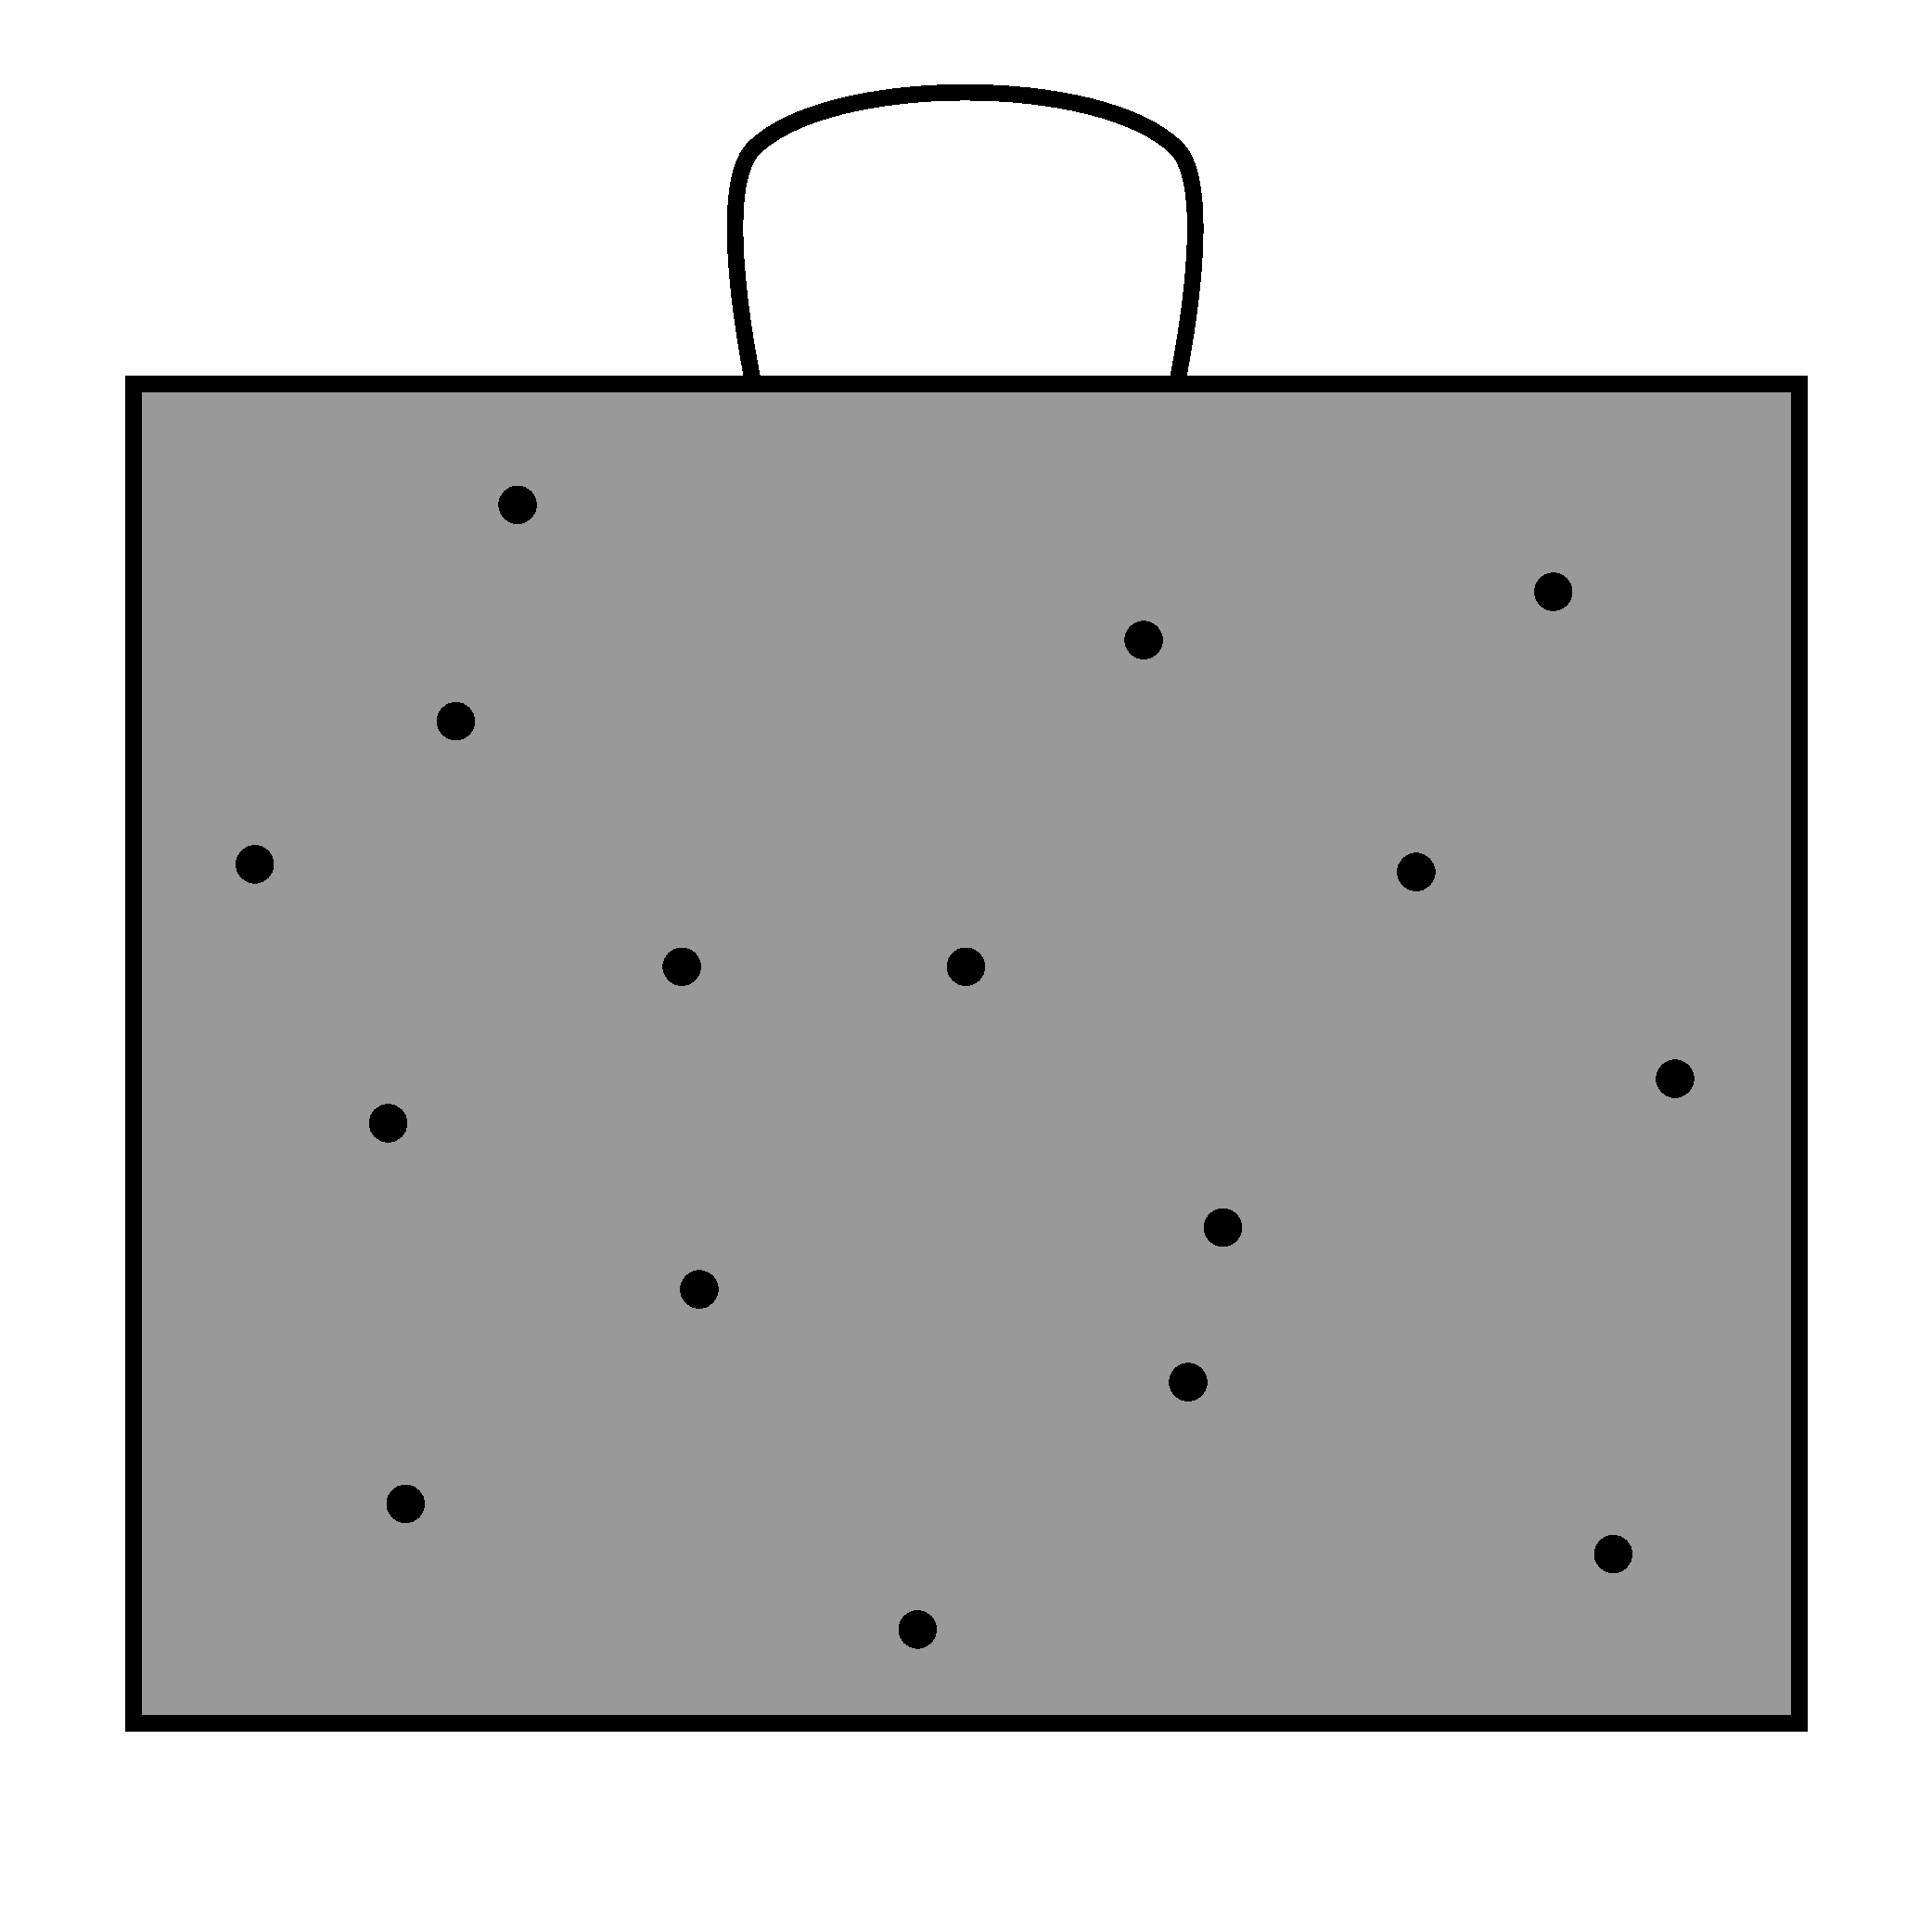
\includegraphics[width=0.4\textwidth]{../figures/olive_oil_can_01.pdf}
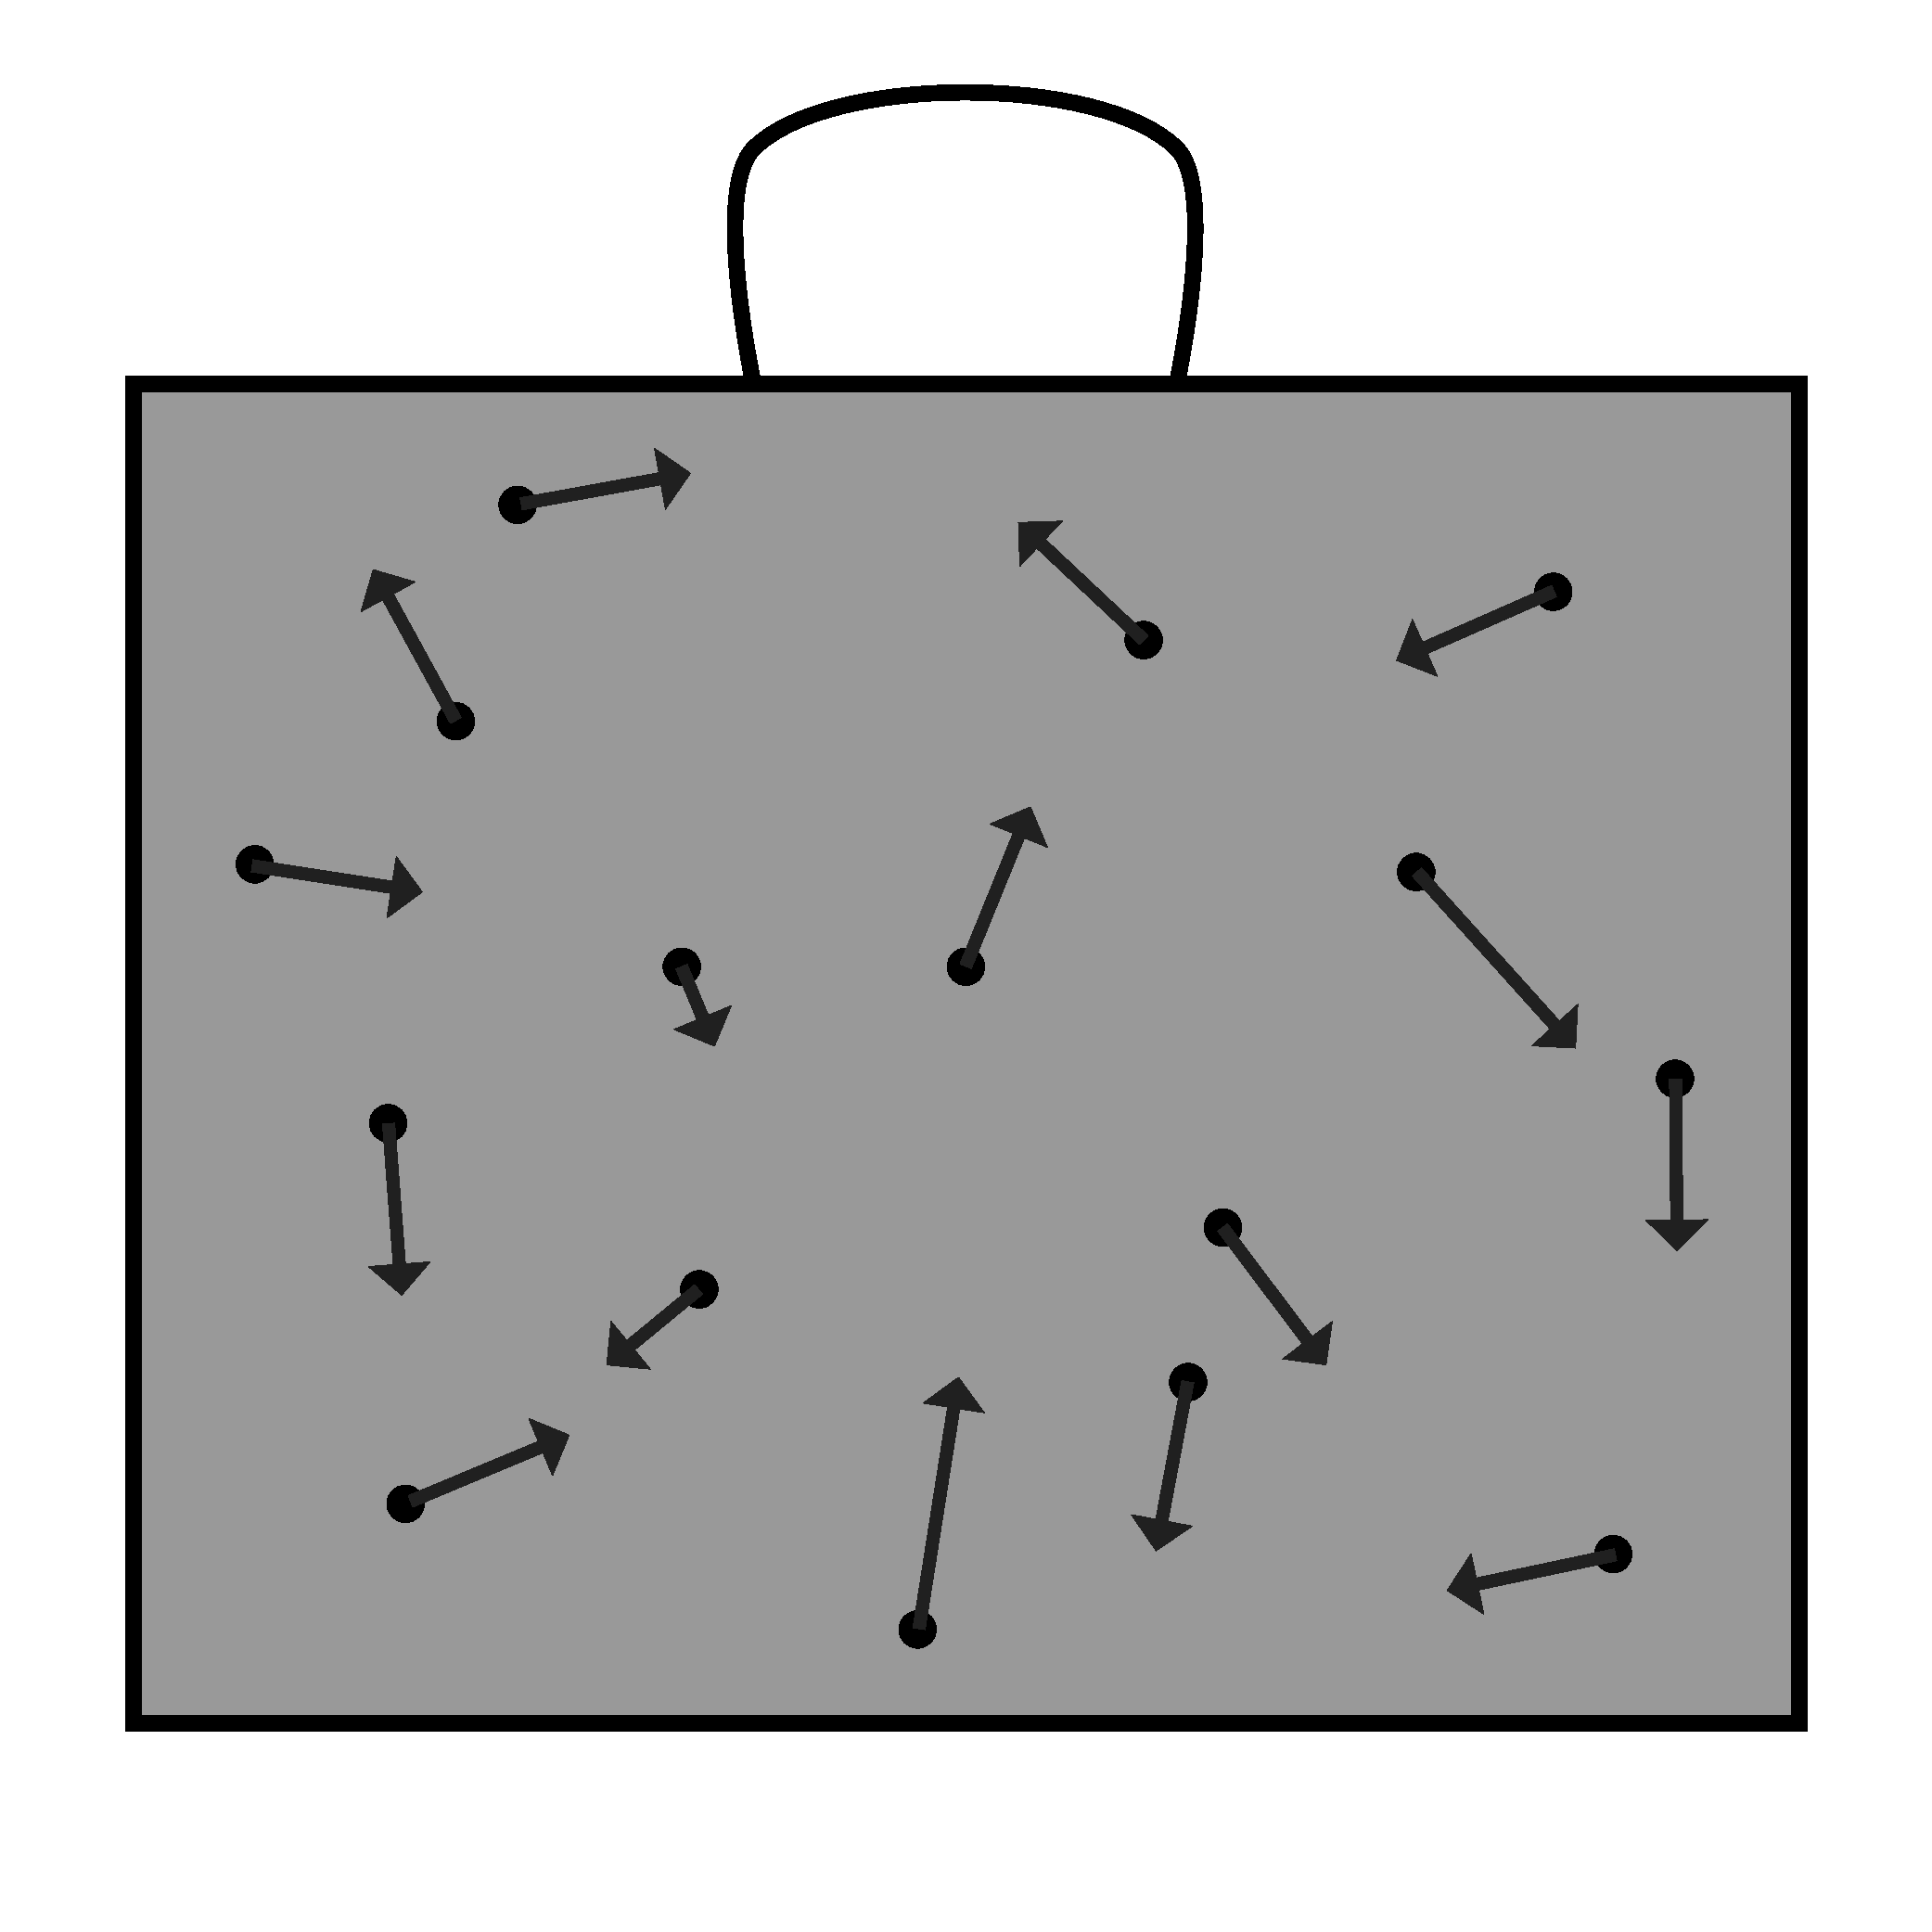
\includegraphics[width=0.4\textwidth]{../figures/olive_oil_can_lagran.pdf}
\caption{Illustration of a glass bottle with Olive oil and spice particles}
\label{fig:Olive_bottle_plain}
\end{figure}

Lagrangian Description lagrangian descr
In the Lagrangian perspective the observer focuses on each separate particle or fluid parcel as it moves inside the glass bottle over time. Therefore the Lagrangian is a material description. Each particle is labelled 
%$p_{i}$ with $i \in \mathbb{N}_{0}$ at the time $t_{0}$ (resting bottle). 
The observer moves with each parcel and measures the physical values like velocity (arrow) or mass of it. These values are recorded for each particle 
%$p_{i}$
. One can consider these particles to be small moving \emph{sensors} that record physical properties of themselves. 

When the recorded information is presented of a property like speed, this might schematically look like the LHS of Figure \ref{fig:lagr_traj}. Each individual particle has the information of speed at a given time. For the observer this already implies that it is possible to know the fate of each particle and its values for the entire observed time. Furthermore one is able to plot the transport pathways, called \emph{pathlines}, of each individual particle in a transport process as depicted on the LHS of Figure \ref{fig:lagr_traj}.

% \begin{figure}[htb]
% \centering
% \begin{tikzpicture}
%     \begin{axis}[
%         xlabel=$Time \ t$,
%         ylabel=$Speed \ s$]
%     \addplot[smooth,mark=*,blue] plot coordinates 
%     {
%         (0,2)
%         (1,5)
%         (2,4)
%         (3,1)
%     };
%     \addlegendentry{$p_{0}$}

%     \addplot[smooth,mark=*,red]
%         plot coordinates 
%         {
%             (0,0)
%             (1,1)
%             (2,1)
%             (3,5)
%         };
%     \addlegendentry{$p_{1}$}

%     \addplot[smooth,mark=*,green] plot coordinates 
%     {
%         (0,4)
%         (1,2)
%         (2,2)
%         (3,2)
%     };
%     \addlegendentry{$p_{2}$}    
%     \end{axis}
%     \end{tikzpicture}
%     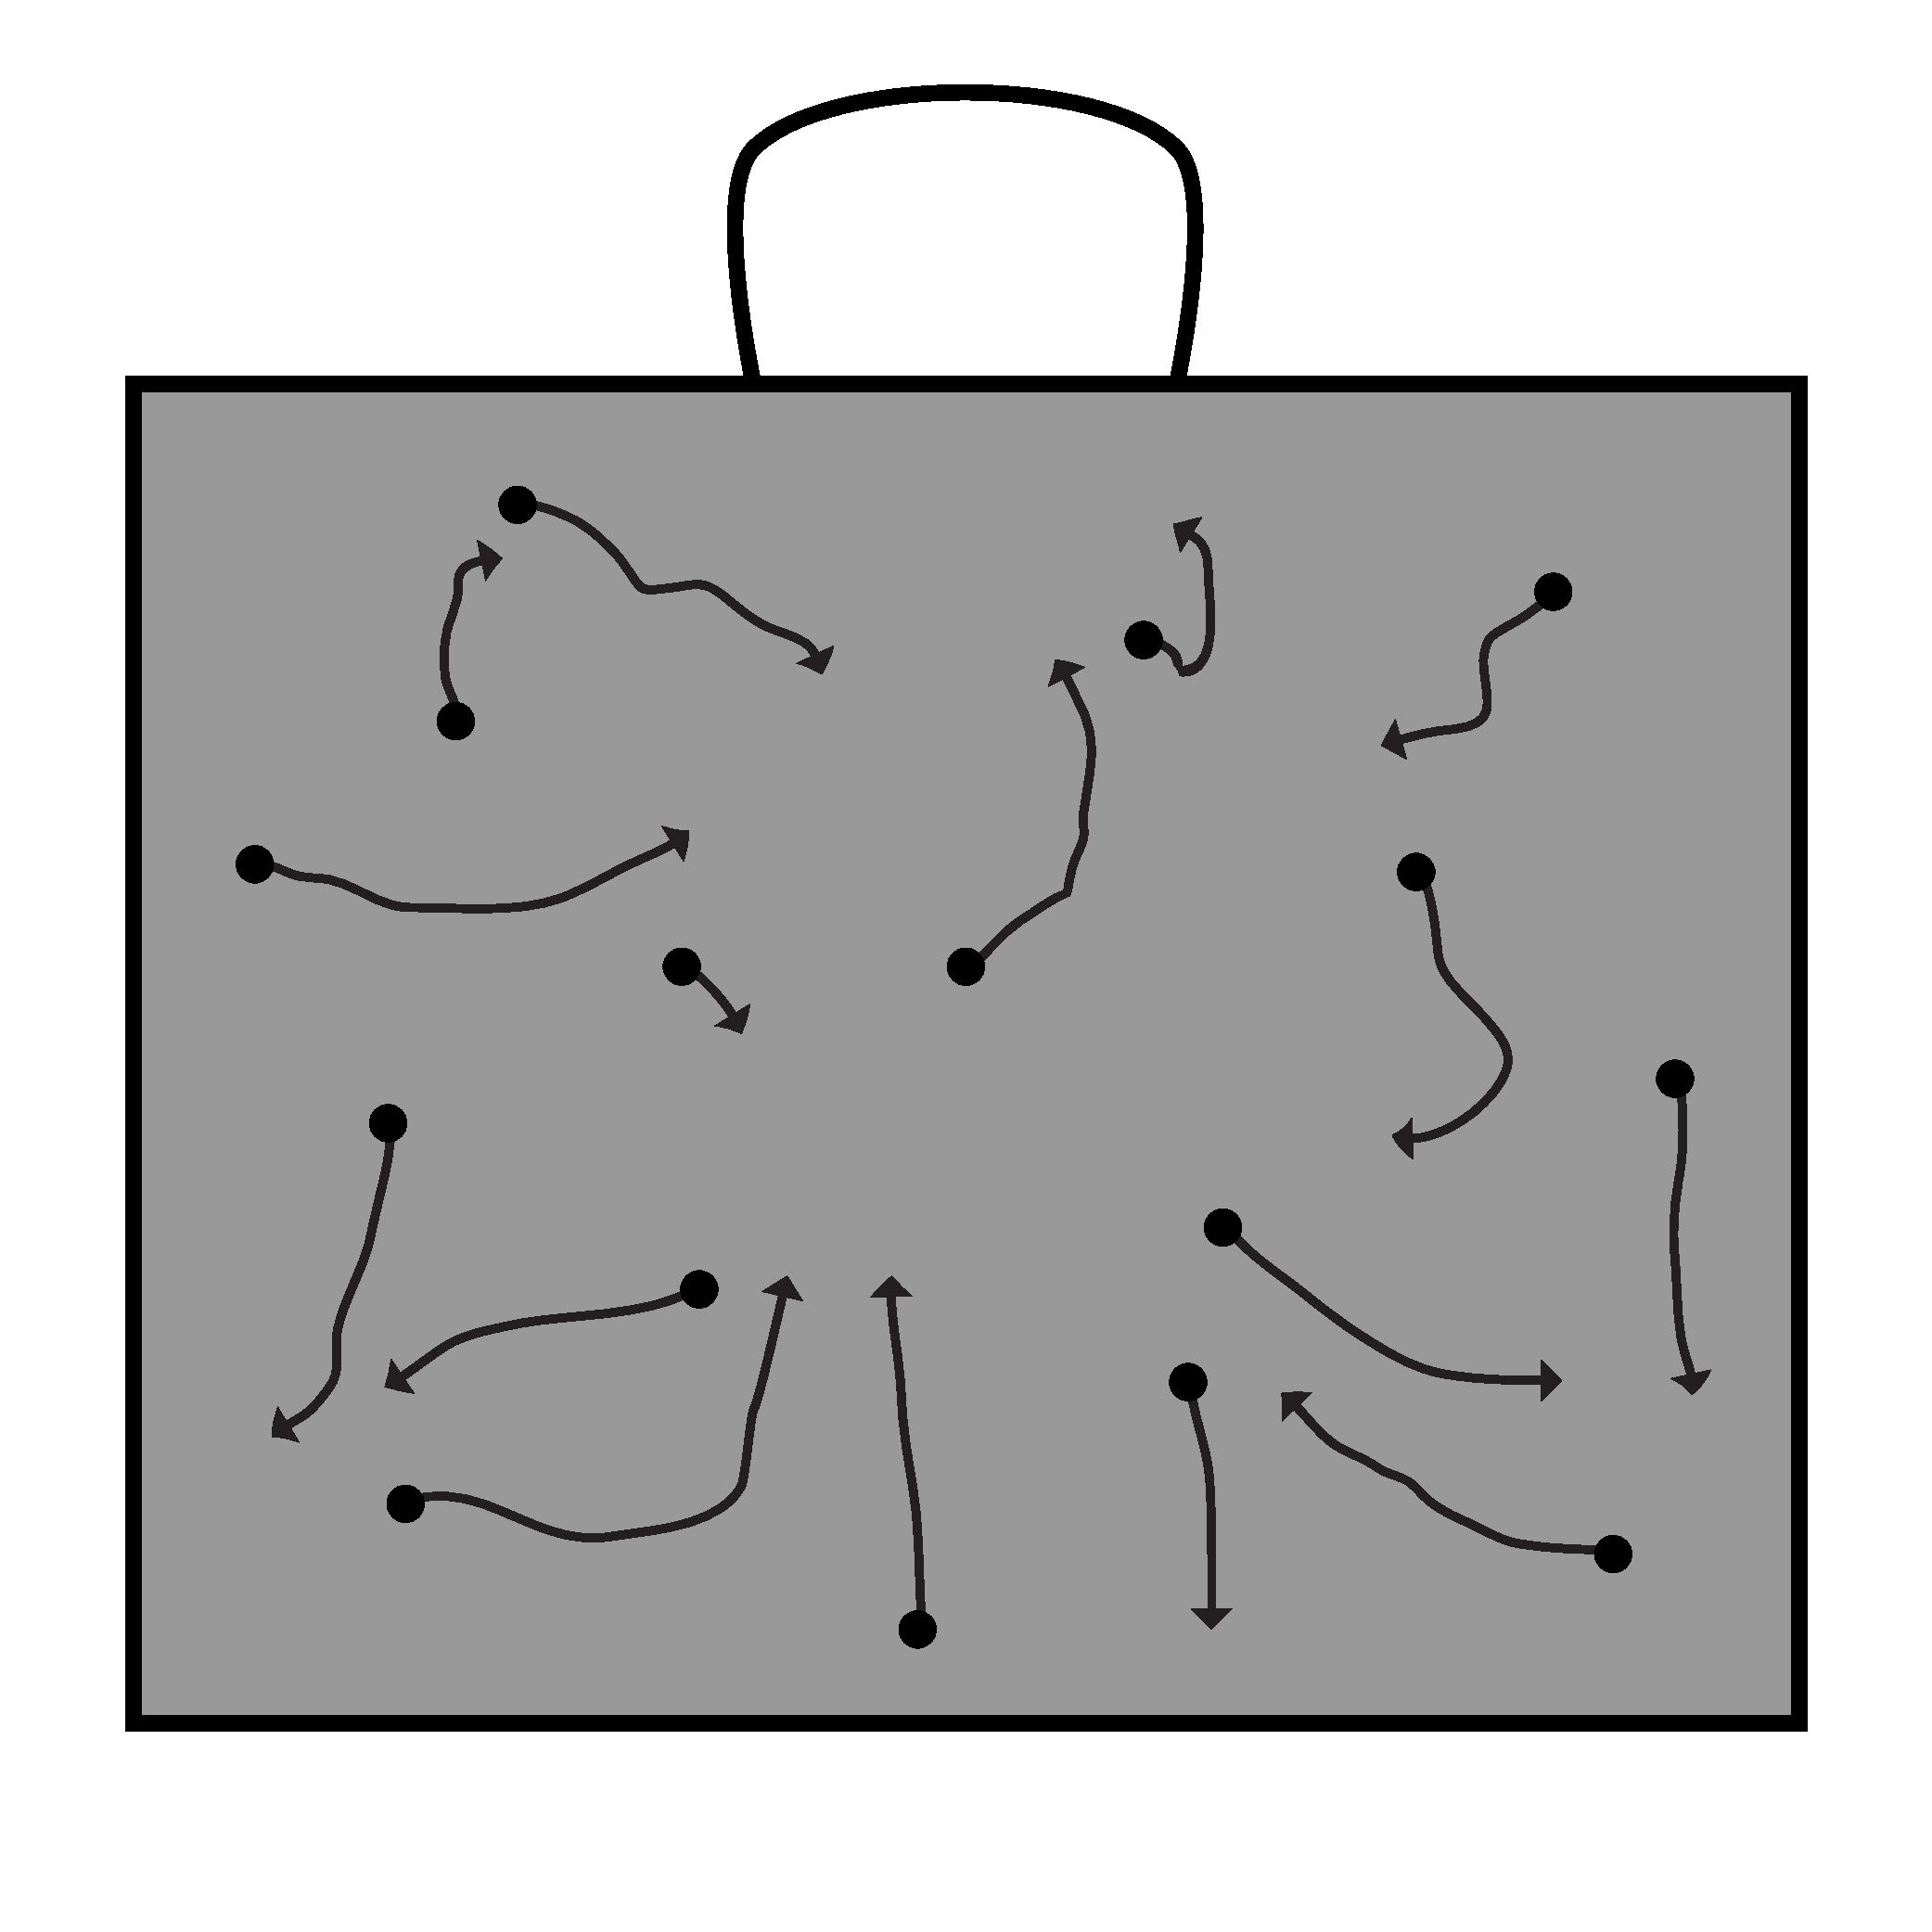
\includegraphics[width=0.4\textwidth]{Figures/olive_oil_can_lagran_pathlines.pdf}
    

% \caption{Schematic diagram of particle's speed and pathlines in Lagrangian perspective}
% \label{fig:lagr_traj}
% \end{figure}



Eulerian Description
eulerian descr

In the Eulerian description the observer does not follow individual fluid parcels. He rather rests and focuses on certain selected locations in the domain of the glass bottle. Therefore the Eulerian is a \emph{spatial} description. To better identify these observation locations, a rectangular mesh is drawn onto the bottle with the intersections being the points of interest. In Figure eulerian bottle observer this is illustrated with hexagonal observer nodes that are located on the intersection points of a rectangular mesh. This mesh discretizes
the spatial domain of the glass bottle (see eulerian mesh). A fluid parcel is only noticed over time and measured by the observer when it passes through a observer node, this is depicted with the red hexagons. So in contrast to the Lagrangian perspective, the \emph{sensors} are static in location. Consequently in the Eulerian the observer is not capable of knowing the trajectories of all fluid parcels.

\begin{figure}[htb]
\centering
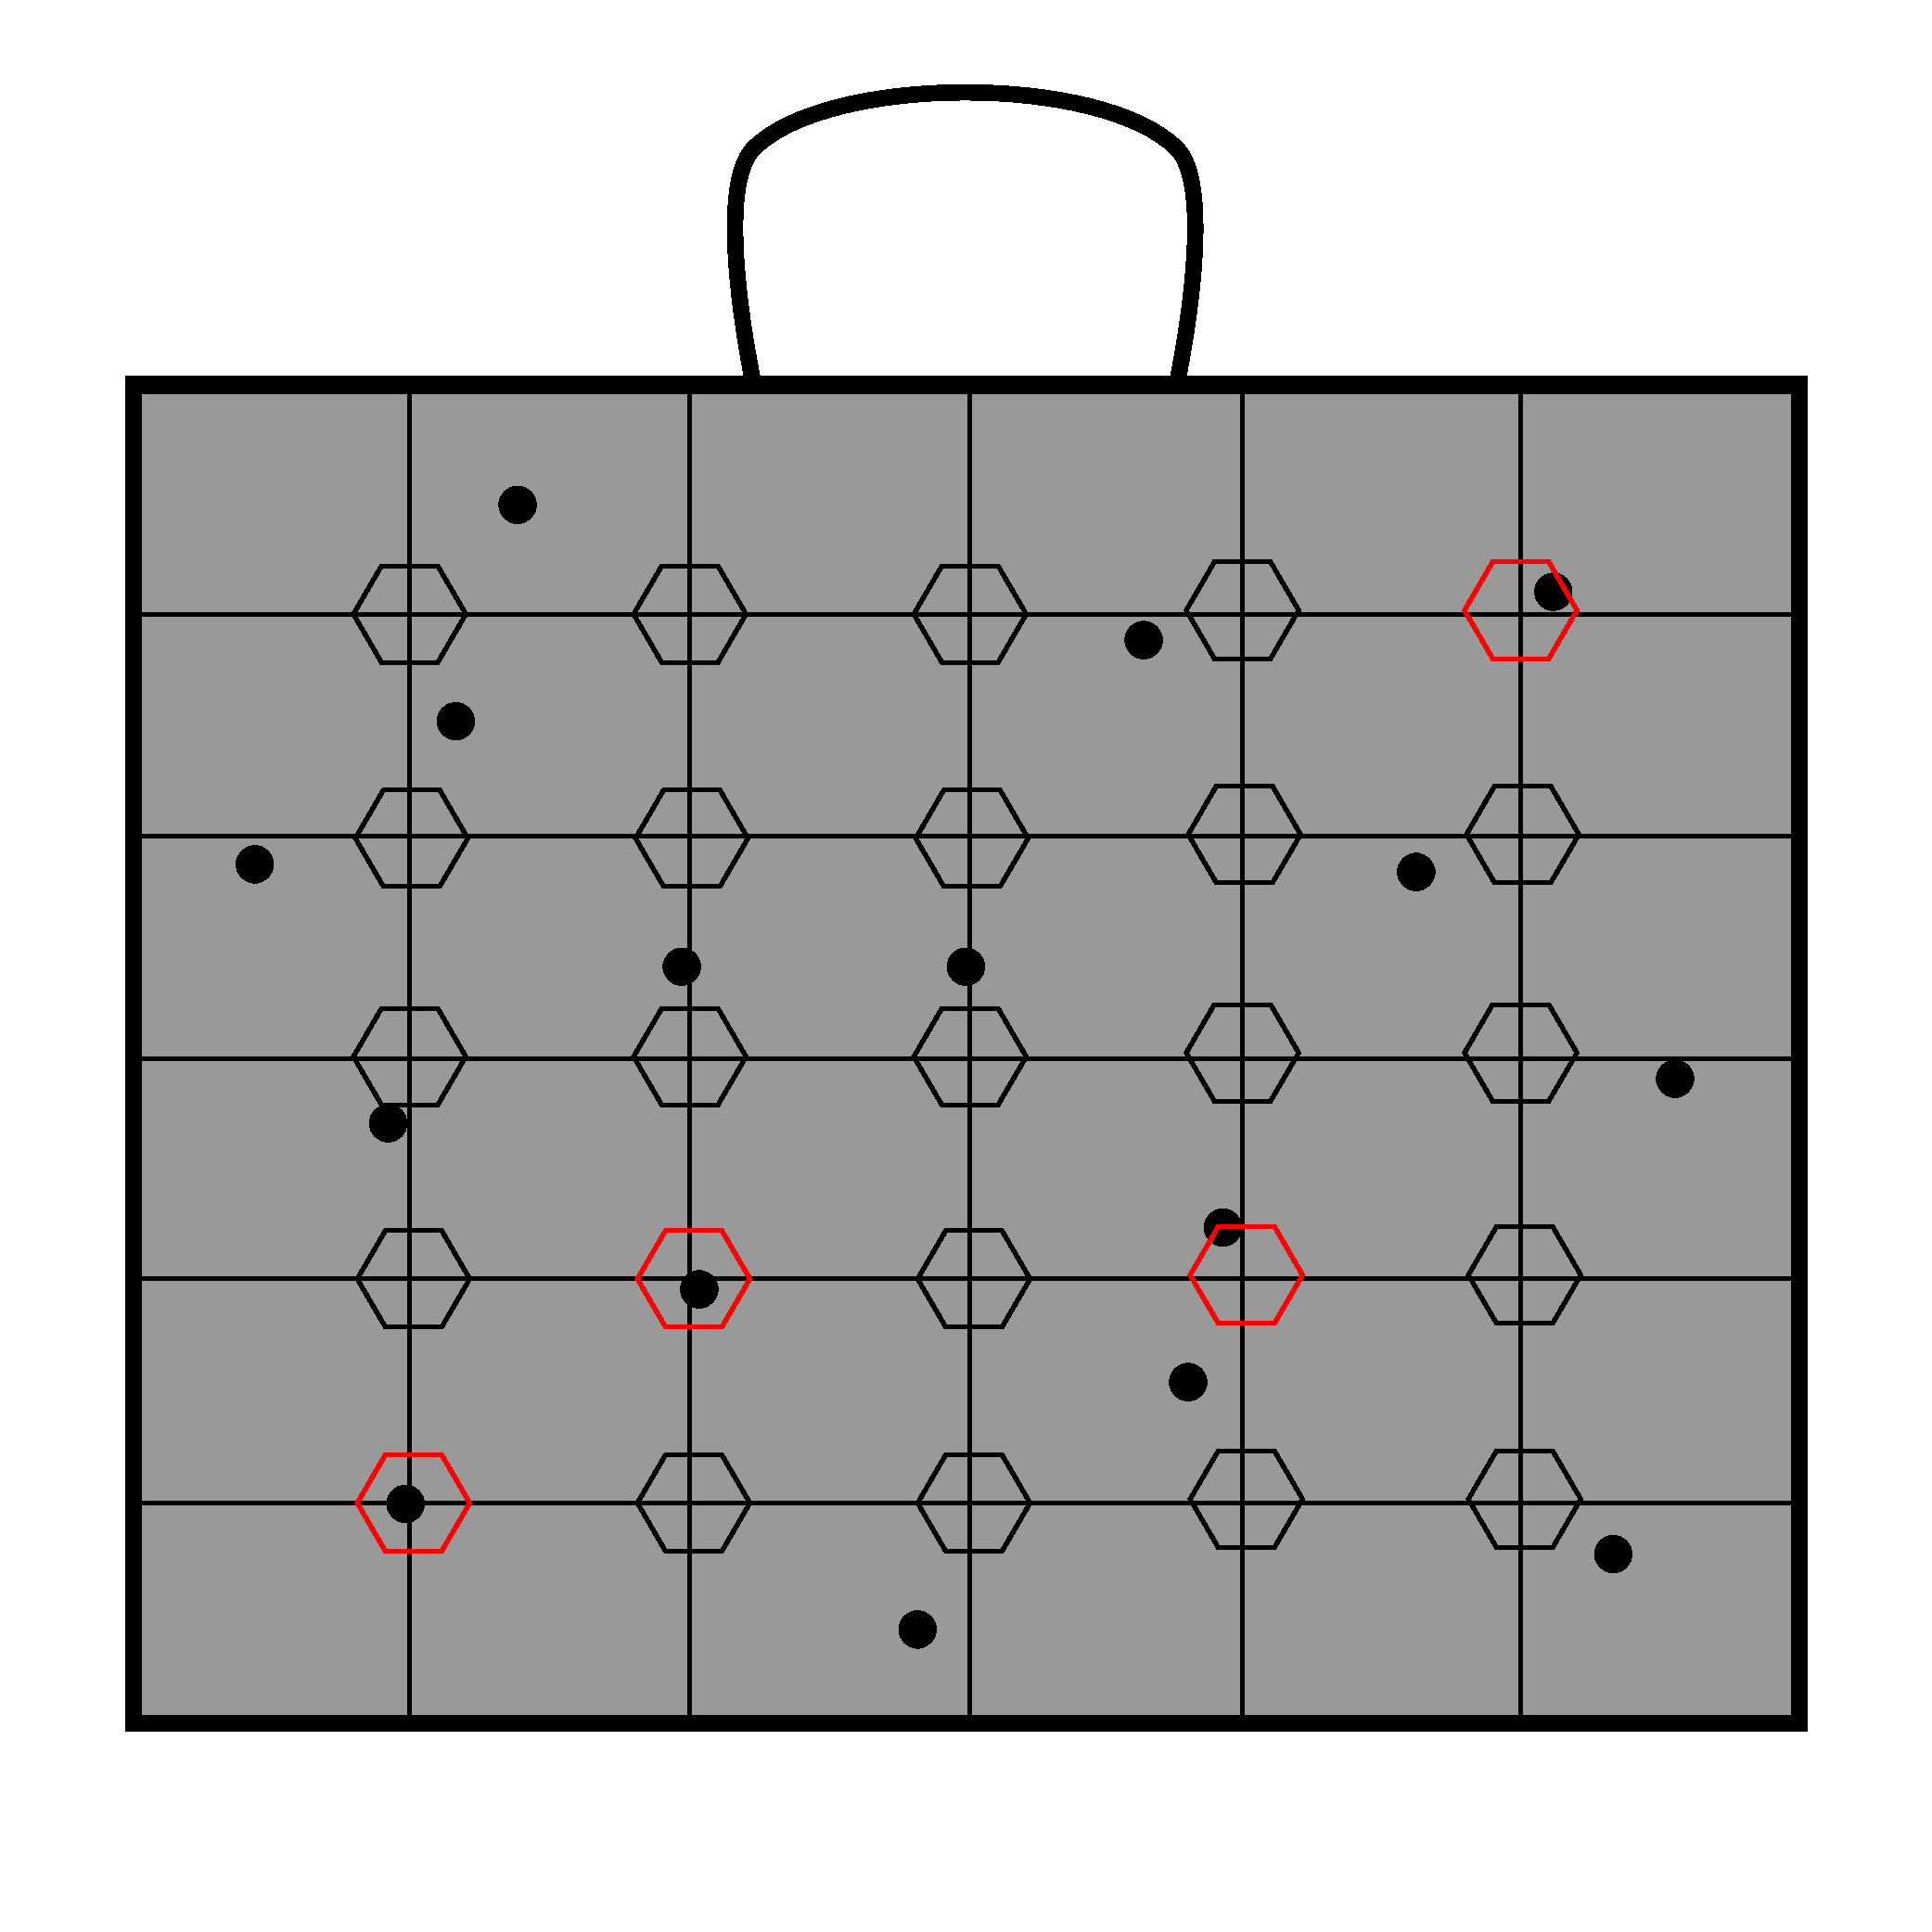
\includegraphics[width=0.4\textwidth]{../figures/olive_oil_can_eulerian.pdf}
\caption{Illustration of hexagonal observer nodes inside a rectangular mesh in Eulerian perspective}
\label{fig:eulerian_bottle_observer}
\end{figure}


\subsection{Lagrangian vs. Eulerian Description}
To bring both descriptions into a mathematical framework we first start with the Lagrangian. As mentioned above each individual particle is labeled $p_{i}$ at time $t_{0}$ when the bottle is released to rest. This label is a vector of the fluid properties or the particles Cartesian coordinates at the time of release. The Lagrangian observer follows the particle after time $t_{0}$ and notes down the position of this individual particle at time t as:

\begin{equation}
X_{i}(p_{j}, t_{0} | t)
\end{equation}

In Eulerian description the position of a observer is simply $x_{i}$. The above situation that this Eulerian observer is able to recognize a fluid parcel (red hexagons) is only given when:

\begin{equation}
x_{i} = X_{i}(p_{j}, t_{0} | t)
\end{equation}

Similar to this the velocity relation in Eulerian and Lagrangian perspective is given by:

\begin{equation}
v(x_{i},t) = \frac{\partial X_{i}}{\partial t} (p_{j}, t_{0} | t)
\end{equation}

Where the LHS denotes the velocity v from the fluid parcel detected by a Eulerian observer, the RHS denotes the Lagrangian version. In similar manner the relation to the rate of change of other physical quantities like heat or momentum can be found. A important mathematical instrument for this is the Stokes derivative, also called material derivative.

\subsection{The Material Derivative}

(Explain the bridge between the eulerian and the langrangian perspective through the material derivative.)

\subsection{Implications on Fluid Dynamics}

In Fluid Dynamics the transport or \emph{flux} of fluids is of primary interest. In Eulerian description the flux can only be estimated correctly when there is a dense spatial and temporal coverage of observing nodes.

Flux processes itself are fundamentally a Lagrangian quantity and therefore easier to describe in this perspective. As we will see in the following Chapters, methods with a Eulerian description like FVM have ways to estimate the flux in a certain region. But with more complicated, even deforming, geometry the Lagrangian description is capable of handling these changes far better (e.g FEM). The Lagrangian is used widely in astrophysics, where the gravity of stars, planets and galaxies interact within a vast space of vacuum without any interesting behaviour. The focus lies here on relatively few objects/parcels in comparison to the immense
spatial distribution of those. Concerning CFD a rough estimation can be already made that the Lagrangian is better for (many) single fluid parcels that are of interest and can have great deformation behaviour. As we will see in this report this is not entirely true. A method in Lagrangian description and a attached mesh can lead to more problems with deformations in CFD than a Eulerian method (see main fem ). In addition
leaving out a mesh in a Lagrangian method, as it is done in Chapter 5, brings out the deformation robustness concerning CFD. For further reading please refer to Bennett2006.

\section{Differential equations diff eq}
In the following Section the gov eq fluiddy are presented. These equations rely heavily on
higher mathematics and describe the fluids properties and flow with various differential equations. This section should brush up very briefly the knowledge on differential equations for the novice reader. Of utmost significance is the classification of partial differential equations into parabolic, hyperbolic and elliptic types, since the later numerical discretization methods are not equally capable of solving all of them efficiently.
\subsection{Ordinary Differential equations}
Ordinary Differential equations (ODE) occur in many CFD terms. Of special interest for this report are they because they are present in the Chapter 5 method.

%Runge Kutta 
\subsection{Partial Differential equations}
%PDEs

\subsection{Divergence theorem}
\label{sec:div_theorem}

\section{Implicit Methods}
\section{Explicit Methods}

\section{Boundary Conditions}
\subsection{Von Neumann Conditions}
\subsection{Dirichlet Conditions}

\section{Governing equations of Fluid Dynamics}

As we have seen in Chapter Chapter2 there are many different types of flow in Fluid Dynamics and many physical properties that define them. As this report focuses on unsteady flow, a key finding of Science is that the \emph{entire} motion and behaviour of a fluid flow can be indicated by the conservation laws for \textbf{momentum}, \textbf{mass} and \textbf{energy}. We will use the already explained general form of conservation laws and apply them to these three properties leading to the Euler equations and Navier-Stokes equations. These equations are of a very general Nature and need supporting physical laws when they are applied to a more specific fluid type like incompress fluid. This can lead to a massive simplification of the NSE, since depending on the nature of the specified fluid type many equations become simpler or even zero out. Moreover also external properties like forces need be considered, when they actually influence the fluid itself. An excellent example of such can be found in Warner2010 where in order to model the behaviour of fluid packets in our atmosphere also the coriolis forces and Earth's gravity influence the fluids momentum. The set of equations are usually coupled to a certain degree, which complicates solving them. 

 

\subsection{Conservation of Momentum}



\subsection{Conservation of Mass}

The conservation of mass is a key property of fluid flow. In a closed fluid system
no mass is created at any point or destroyed. This fact is of great use later on in FVM were withing a subdivided discrete volume no material sources or sinks exists.
The physical changing value of the fluid's density $\rho$ is bound by this law in the overall system. The fluids mass only is transported by convective flux, which considering the above notations of a conservation law leads to:

\begin{equation}\label{eq:con_mass_1}
\frac {\partial}{\partial t} \int\limits_{\Omega} \rho d \Omega +
\oint\limits_{A} \rho \vec{v} \cdot d \vec{A} = 0
\end{equation}



\subsection{Conservation of Energy}





Mathematical model of fluid motion
Form? integral form ...auch sections machen?

\subsection{Euler equations}
The Euler equations don't cover viscosity and any kind of heat conduction effects. They are of hyperbolic nature in space and time. Therefore these equations only cover invisicid flow of fluids.

\begin{equation}
\rho \frac{dv}{dt} = 
\rho ((\nabla \cdot v)\cdot v + \frac {\delta v}{\delta t }) =
f - \nabla p 
\end{equation}


\subsection{Navier-Stokes equations}
\label{sec:NSE_main}
The Navier-Stokes equations (NSE) are a set of equations to describe (in)compressible
viscous fluid flows. Therefore they can be seen as a extension and a more accurate version of the Euler equations that now include viscosity and heat conduction. Formulated by the French physicist Claude-Louis Navier with contributions from the Irish physicist George Stokes in the 19th century these set of equations are the cornerstones of today's understanding of fluid dynamics. The set of Navier-Stokes equations are in general parabolic equations in time and space. 

%Assumptiuons and preconditions


%Initial conditions
%Boundary conditions
%Numerical Solver to solve the equations

 

%Continuum laws



%In Fluid Mechanics 
%page 116



